\talksection{Scalarization Stage}

\begin{frame}[fragile]{Scalarization Overview}

\begin{itemize}
    \item Eliminates vector operations from the source function
    \item Vector types used likely to be narrower than the native SIMD width
    \item Combining scalarization with packetization
    \begin{itemize}
        \item Generate vector instructions with the native SIMD width
        \item Implicitely performs 'Structure-of-Arrays to Array-of-Structures' conversion
    \end{itemize}
    \item Alternative is instantiating vector instructions (and users) $N$ times
    \item Example: Extract audio samples  from left and right channels, scale by $\frac{1}{2}$
\end{itemize}

\begin{codebox}[commandchars=\\\[\]]
global int2 \uniform[*src], int \uniform[*left], int \uniform[*right];
int \varying[tid] = \varying[get_global_id(0)];
int2 \varying[sample] = \uniform[src]\idx[\varying[tid]];
\uniform[left]\idx[\varying[tid]] = (\varying[sample.x] >> \uniform[1]);
\uniform[right]\idx[\varying[tid]] = (\varying[sample.y] >> \uniform[1]);
\end{codebox}

\end{frame}

%%%%%%%%%%%%%%%%%%%%%%%%%%%%%%%%%%%%%%%%%%%%%%%%%%%%%%%%%%%%%%%%%%%%%%%%%%%%%%%%

\begin{frame}{Scalarization Process}

\begin{itemize}
    \item Look for vector \varying{varying} instructions such as:
    \begin{itemize}
        \item Leaves that define vector values, vector stores
        \item Vector extractions
        \item Vector -> scalar bitcasts
    \end{itemize}
    
    \item Recursively scalarize until we reach a scalar value
    \begin{itemize}
        \item Operands before instructions
        \item Re-create instructions for each vector element
        \item Vector lane $\neq$ SIMD instance!
    \end{itemize}
    
\end{itemize}

\end{frame}

%%%%%%%%%%%%%%%%%%%%%%%%%%%%%%%%%%%%%%%%%%%%%%%%%%%%%%%%%%%%%%%%%%%%%%%%%%%%%%%%

\begin{frame}[c]{Scalarization Example: Before}

\center{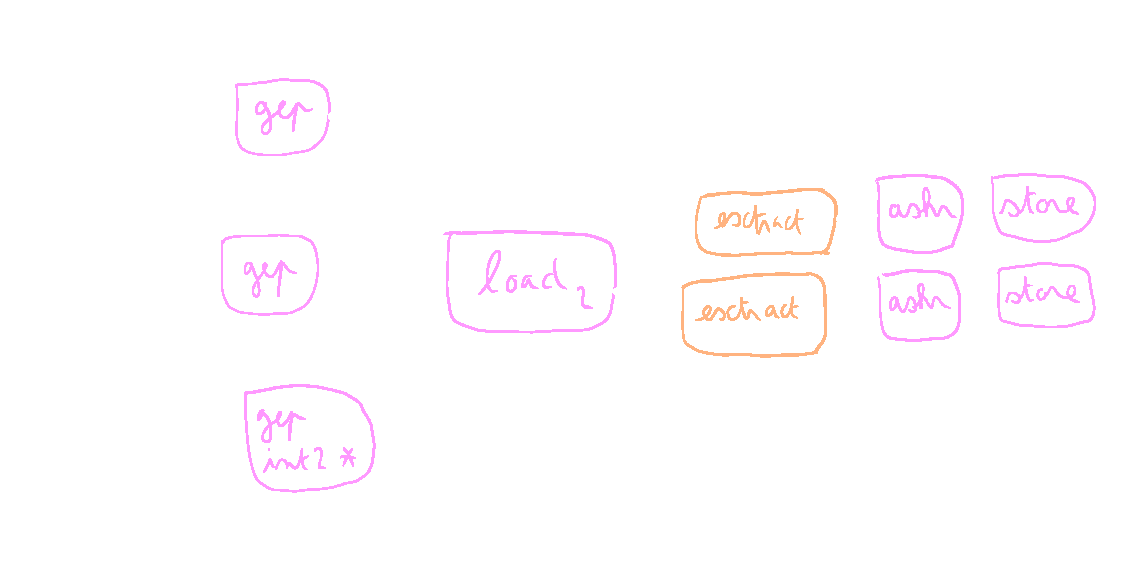
\includegraphics[scale=0.65]{images/scalarization-start.pdf}}

\end{frame}

%%%%%%%%%%%%%%%%%%%%%%%%%%%%%%%%%%%%%%%%%%%%%%%%%%%%%%%%%%%%%%%%%%%%%%%%%%%%%%%%

\begin{frame}{Scalarization Example: After}

[ IR Graph After ]

\end{frame}

%%%%%%%%%%%%%%%%%%%%%%%%%%%%%%%%%%%%%%%%%%%%%%%%%%%%%%%%%%%%%%%%%%%%%%%%%%%%%%%%

\begin{frame}[fragile]{Scalarization Example: IR}

Before Scalarization:
\begin{codebox}
kernel void extract_lr(global int2 *src, global int *left, global int *right) {
    int tid = get_global_id(0);
    int2 sample = src[tid];
    left[tid] = (sample.x >> 1);
    right[tid] = (sample.y >> 1);
}
\end{codebox}

After Scalarization:
\begin{codebox}
kernel void extract_lr(global int2 *src, global int *left, global int *right) {
    int tid = get_global_id(0);
    int sampleLeft = *((int *)&src[tid] + 0);
    int sampleRight = *((int *)&src[tid] + 1);
    left[tid] = (sampleLeft >> 1);
    right[tid] = (sampleRight >> 1);
}
\end{codebox}

\end{frame}

%%%%%%%%%%%%%%%%%%%%%%%%%%%%%%%%%%%%%%%%%%%%%%%%%%%%%%%%%%%%%%%%%%%%%%%%%%%%%%%%

\begin{frame}[fragile]{Scalarization Example}

After Scalarization:
\begin{codebox}
kernel void extract_lr(global int2 *src, global int *left, global int *right) {
    int tid = get_global_id(0);
    int sampleLeft = *((int *)&src[tid] + 0);
    int sampleRight = *((int *)&src[tid] + 1);
    left[tid] = (sampleLeft >> 1);
    right[tid] = (sampleRight >> 1);
}
\end{codebox}

After Packetization:
\begin{codebox}
kernel void extract_lr(global int2 *src, global int *left, global int *right) {
    int tid = get_global_id(0);
    int4 samplesLeft  = interleaved_load_int4((int *)&src[tid] + 0, 2);
    int4 samplesRight = interleaved_load_int4((int *)&src[tid] + 1, 2);
    ((int4 *)left)[tid / 4] = (samplesLeft >> 1);
    ((int4 *)right)[tid / 4] = (samplesRight >> 1);
}
\end{codebox}

\end{frame}
